\subsubsection{Mobaka-Gruppe}\label{sec:MKA-Gr}

Entlang des \mbox{Likwala}-\mbox{aux}-\mbox{Herbes} sowie des Unterlaufs des \mbox{Sangha} fand sich eine weitere Gruppe rezenter Keramik, welche sich vor allem durch rundbodige Knickwandschalen des Typs F3 auszeichnet. Insgesamt können 79~GE dieser nach der Fundstelle Mobaka am unteren \mbox{Sangha} (Fpl.~246) benannten Stilgruppe zugerechnet werden. Überdies wurden 23 Scherben ausgezählt erfasst. Randscherben, die 80\,\% aller Stücke ausmachen, sind in so großer Zahl im Inventar der Mobaka-Gruppe vertreten, da ausbiegende Ränder mit einem innenseitig scharfen Umbruch eines der wenigen diagnostisches Merkmals der Stilgruppe sind. Daneben fanden sich acht komplette oder hinreichend komplette Gefäße. Einige Wandungsfragmente konnten -- vornehmlich aufgrund ihre Bemalung mit vertikalen, dunklen Streifen -- der Mobaka-Gruppe zugerechnet werden. Die Zuordnung zu dieser Stilgruppe konnte in 70\,\% aller Fälle sicher vorgenommen werden. Funde der Mobaka-Gruppe sind von 21 Fundplätzen bekannt, vor allem entlang des \mbox{Likwala}-\mbox{aux}-\mbox{Herbes} sowie des unteren \mbox{Sangha}. Aus Gombe am Kongo (Fpl.~237) liegen zwei möglicherweise der Mobaka-Gruppe zurechenbare GE vor. Das Gros der Funde stammt aus Yumba (Fpl.~289), Botwale (Fpl.~286), Boleko (Fpl.~292), Misongo (Fpl.~288) sowie Bojenjo (Fpl.~292). Alle diese Fundstellen erbrachten je mindestens zehn GE der Mobaka-Gruppe, wobei sich in Yumba mit 26~GE die meisten Stücke fanden. Die maßgebende Beschreibung der Charakteristika der Mobaka-Gruppe erfolgte jedoch anhand eines kompletten Gefäßes aus der namensgebenden Fundstelle Mobaka am untere \mbox{Sangha} (Fpl.~246; Abb.~\ref{fig:MKA-Typen}.1).


\paragraph{Technologische Merkmale}\hspace{-.5em}|\hspace{.5em}%
Die Keramik der Mobaka-Gruppe wurde in der Regel aus weißbrennenden Tonen hergestellt (65\,\%). Lediglich in wenigen Fällen ließen sich Stücke beobachten, die aus rotbrennenden Tonen gearbeitet sind (12\,\%). Bei einer größeren Anzahl GE (23\,\%) ließ sich aufgrund ihrer beigen, grauen bis schwarzen Färbung die Brennfarbe der Tone nicht sicher ansprechen. Die GE enthalten so gut wie keine (69\,\%) oder nur sehr wenige (22\,\%) nichtplastische Partikel. Sind Partikel sichtbar, so handelt es sich für gewöhnlich um homogene Quarzsande (82\,\%), welche vor allem in der Korngrößenklasse \textit{very fine} (50\,\%) vorliegen. Teilweise finden sich jedoch auch größere Partikel der Größenklassen \textit{fine} (21\,\%), \textit{medium} (24\,\%) sowie vereinzelt auch \textit{coarse} (6\,\%). In nur sehr wenigen Fällen enthalten die Stücke mehr als reine Quarzpartikel: Laterit (11\,\%) oder Organik (4\,\%). Daraus folgt, dass sich das Gros der Mobaka-Keramik dem \textit{Fabric} 1 zurechnen lässt (88\,\%). Die \textit{Fabrics} 1b und 1d machen zusammen zwei Drittel (66\,\%) aller GE der Mobaka-Gruppe aus. In geringem Maße finden sich auch Stücke, welche dem rötlich-brennenden \textit{Fabric} 2 angehören sowie jeweils ein Stück der \textit{Fabrics} 3c und 4a. Die Oberflächen der Stücke sind fast ausschließlich glatt (75\,\%), nur sehr wenige Stücke zeigen eine leicht raue Oberfläche (5\,\%), welche sich aber in jeweils einem der Fälle nur auf die Innen- oder Außenseite beschränkt. Die Dicke der Gefäßwandungen liegt im Mittel bei 6,6\,mm, jedoch wurden auch einige Stücke mit deutlich stärkeren Wandungen beobachtet.

\begin{figure*}[p]
	\centering
	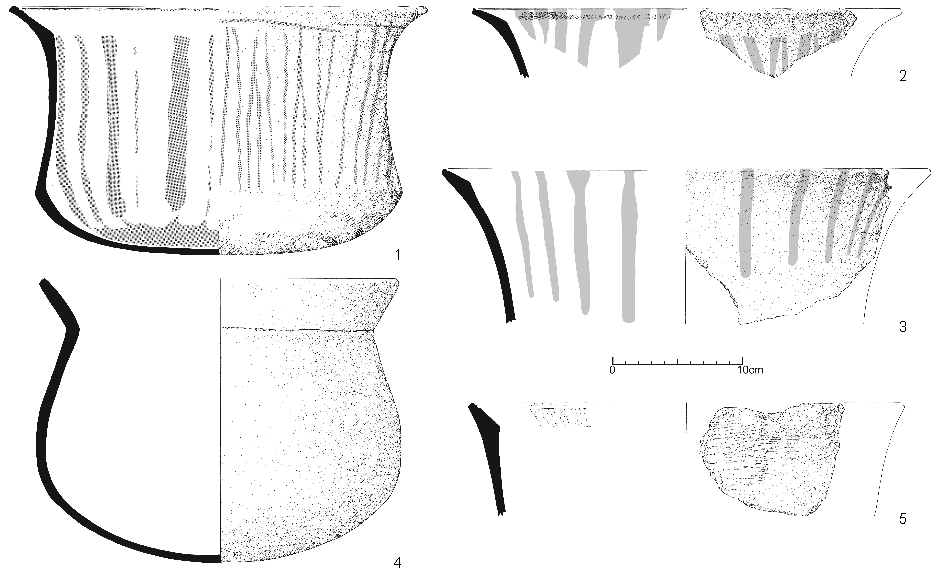
\includegraphics[width=\textwidth]{fig/MKA-Typen.pdf}
	\caption{Mobaka-Gruppe: Typvertreter.\\ 1:~Taf.~39.1; 2:~Taf.~73.3; 3:~Taf.~74.7; 4:~Taf.~68.4 (Reste von Bemalung aus vertikalen, dunklen Streifen wie 1--3, nicht abgebildet); 5:~Taf.~74.8.}
	\label{fig:MKA-Typen}
\end{figure*}

\begin{figure*}[p]
	\centering
	\begin{subfigure}{\columnwidth}
		\centering
		\includegraphics[width = \columnwidth]{fig/BOO87-101_HH87-II-18-27.jpg}
		\caption{Bondo (Fpl.~245; Foto: H.~Holsten, 1987).}
		\label{fig:BOO87-101}
	\end{subfigure}\hfill
	\begin{subfigure}{\columnwidth}
		\centering
		\includegraphics[width = \columnwidth]{fig/MIS87-101_E87-029-14_b.jpg}
		\caption{Misongo (Fpl.~288; Foto: M.~K.~H.~Eggert, 1987).}
		\label{fig:MIS87-101_Detail}
	\end{subfigure}
	\caption{Mobaka-Gruppe: Im Gelände beobachtete, rezente Schalen des Typs F3. Die beiden Gefäße in Bondo am \mbox{Sangha} (Fpl.~245; \textbf{A}) sollen Berichten der lokalen Bevölkerung nach aus Bamataba am \mbox{Sangha} stammen. Eine Fotografie einer Feuerstelle in Misongo am \mbox{Likwala}-\mbox{aux}-\mbox{Herbes} (Fpl.~288; \textbf{B}) zeigt tönerne, zuckerhutförmige Feuerböcke sowie eine Schale des Typs F3 mit Metalldeckel.}
	\label{fig:rezenteMBK-Schalen}
\end{figure*}

\begin{figure*}[p]
	\centering
	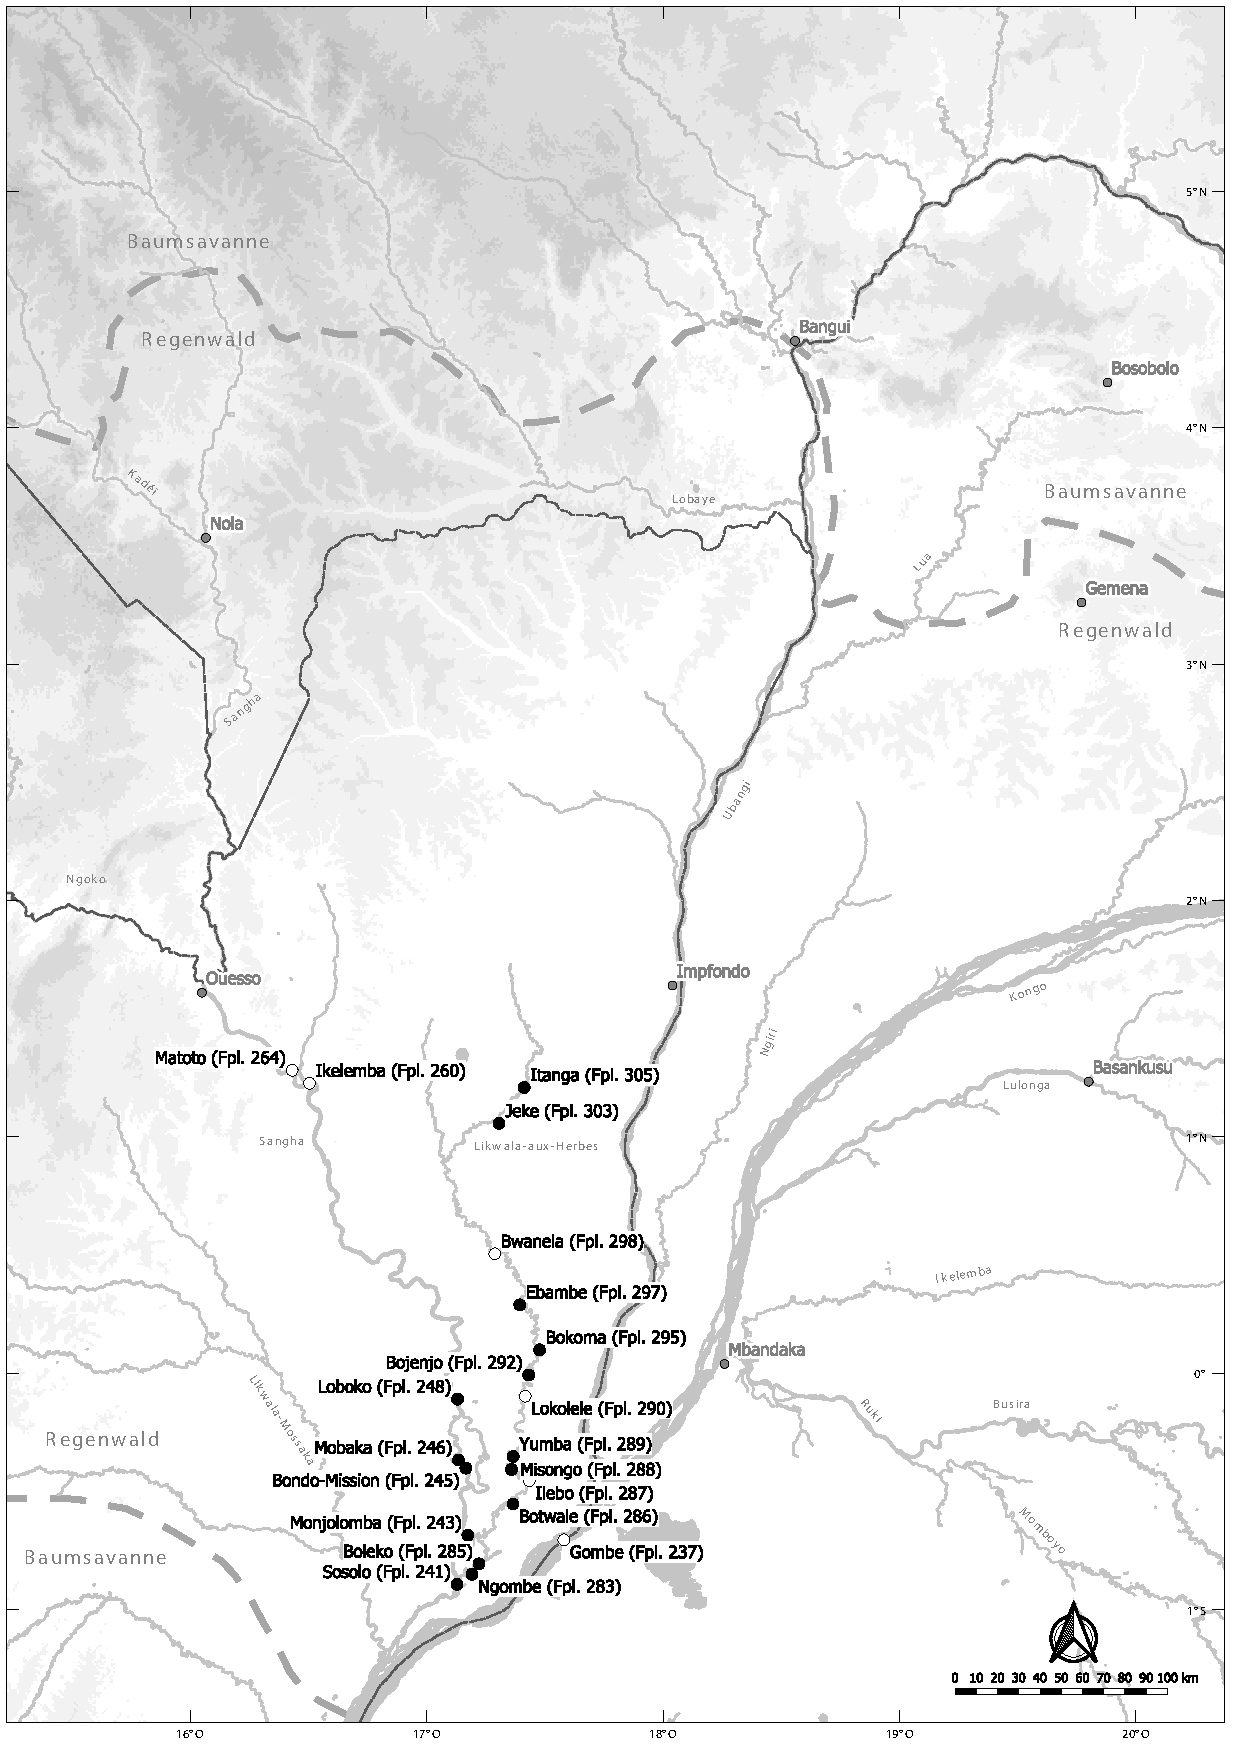
\includegraphics[width=\textwidth]{fig/MKA_Verbreitung.pdf}
	\caption{Mobaka-Gruppe: Verbreitung.}
	\label{fig:MKA_Verbreitung}
\end{figure*}

\paragraph{Formen}\hspace{-.5em}|\hspace{.5em}%
Bei insgesamt 22 von 41~GE konnte die Gefäßform sicher bestimmt werden. Bei 33~GE und damit dem überwiegenden Teil handelt es sich um Schalen mit scharfem Bauchknick vom Typ F3 (78\,\%; Abb.~\ref{fig:MKA-Typen}.1--3,5). Die Schalen weisen maximale Durchmesser zwischen 11--32\,cm auf, während die Mündungen zwischen 6--50\,cm weit sind. Die Höhe der Mündung liegt zwischen 6,5--21\,cm. Die sich daraus ergebenden Proportionen der Mündungshöhe zum maximalen Durchmesser, der häufig auch durch den Mündungsdurchmesser gegeben ist, liegt bei zirka 1:1,8. Die Schalen sind folglich häufig fast doppelt so breit wie hoch. Die Bestimmung der Mobaka-Gruppe fußt zu großen Teilen auf den beschriebenen Schalen des Typs F3. Daneben wurden charakteristische Ränder mit innen liegendem scharfen Umbruch sowie die Bemalung mit vertikalen Streifen, welche sich aber nur auf einigen der Schalen findet, für die Zuweisung zur Mobaka-Gruppe herangezogen. Selten konnten andere Gefäßformen der Mobaka-Gruppe zugeordnet werden. So fand sich in Grab BLK~87/1 in Boleko, an der Mündung des \mbox{Likwala}-\mbox{aux}-\mbox{Herbes} (Fpl.~285), ein Gefäß mit geschweifter Wandung und einfach ausbiegendem Rand vom Typ E1, das aufgrund einer äußeren Bemalung mit dunklen, vertikalen Streifen, die ansonsten nur die genannten Schalen der Mobaka-Gruppe zeigen (Abb.~\ref{fig:MKA-Typen}.1--3), der Stilgruppe zugerechnet wird (Abb.~\ref{fig:MKA-Typen}.4). 

Bei 67~GE der Mobaka-Gruppe war der Rand erhalten. Die Mobaka-Gefäße werden von ausbiegenden Formen mit einem innenseitigen scharfen Umbruch bestimmt (B1.5; 77\,\%). Darüber hinaus sind lediglich einfach ausbiegende Ränder vom Typ B1 beobachtet worden. Die Randlippe ließ sich bei insgesamt 58~GE beobachten, sie ist größtenteils schräg nach außen abgestrichen (M5; 67\,\%), in seltenen Fällen aber auch spitz ausgeformt (14\,\%) oder gerade abgestrichen (7\,\%). Die schräg nach außen abgestrichenen Randlippen finden sich regelhaft und fast ausschließlich an den ausbiegenden Rändern mit innenseitigem Profilknick vom Typ B1.5. Aufgrund des Mangels an GE, welche nicht der Schalenform F3 zuzurechnen sind, fehlen GE mit ausgearbeiteten Hals- und Schulterzonen im Inventar der Mobaka-Gruppe vollständig. Die insgesamt 17~GE, bei denen eine Ansprache der Bodenform möglich war, zeigten entweder eine runde Standfläche (B1; 88\,\%) oder einen Linsenboden (B2; 12\,\%). Flache Böden konnten nicht beobachtet werden.

\paragraph{Verzierungen}\hspace{-.5em}|\hspace{.5em}%
Mobaka-Keramik weist häufig nur horizontale Rillen (Tab.~\ref{tab:Verzierungselemente}: 02.1) auf, die knapp die Hälfte aller aufgenommenen Verzierungselemente ausmachen und bis auf wenige Ausnahmen fast durchweg auf der Innenseite der Ränder des Typs B1.5 zu finden sind (Abb.~\ref{fig:MKA-Typen}.1--3,5; Anlage~4\subref{fig:MKA_Verz}). Daneben fallen Bemalungen der Innen- sowie Außenseiten mit vertikalen, dunklen Streifen auf (Tab.~\ref{tab:Verzierungselemente}: 14.1; 26\,\%; Abb.~\ref{fig:MKA-Typen}.1--3). Gelegentlich konnte auch \textit{banfwa-nfwa}-Verzierung auf den Innenseiten sowie außen am Gefäßbauch und den Standflächen beobachtet werden (Tab.~\ref{tab:Verzierungselemente}: 08; 11\,\%; Abb.~\ref{fig:MKA-Typen}.1,5). Die Verzierung findet sich vor allem an der Innenseite der Gefäßränder (52\,\%). Deutlich seltener sind Gefäßwandungen verziert (22\,\%). Bei zwei GE findet sich Verzierung auch auf den Standflächen.

\paragraph{Datierung}\hspace{-.5em}|\hspace{.5em}%
Für die Keramik der Mobaka-Gruppe liegen keine absoluten Datierungen vor, jedoch weisen Fotos entsprechender GE, die während der Prospektionen am \mbox{Sangha} und \mbox{Likwala}-\mbox{aux}-\mbox{Herbes} 1987 gemacht wurden, auf ein rezentes Alter hin (Abb.~\ref{fig:rezenteMBK-Schalen}). Eine rundbodige Schale mit Bauchknick, leicht konkavem Oberteil und vertikaler Bemalung -- die \textit{Leitform} der Mobaka-Gruppe -- aus dem Bereich des Pool Malebo \parencite[150, Taf.~XI.171]{Coart.1907}, findet sich in der umfangreichen Vorlage ethnografischer Funde des \textit{Musée royal de l'Afrique centrale} in Tervuren\footnote{Das Museum trug seinerzeit den Namen \textit{Musée du Congo} (heute \textit{Musée royal de l'Afrique centrale}). Die Gefäße sind als \enquote{Poteries des Bateke, Babuma} beschriftet (\textsc{Anonymus} 1907: Taf. XI).}. Ebenfalls wird eine stark bauchige Flasche aus Kwamouth (ebd. 150, Taf.~XI.172), an der Mündung des Kasai-Flusses in den Kongo, abgebildet, welche eine identische Bemalung zeigt und dem Gefäßtyp A2 entspricht, im hier vorgelegten Material jedoch so nicht beobachtet werden konnte. Eine weitere Schale mit Bauchknick, konkavem Oberteil und gegenständiger Durchlochung unterhalb des Randes, durch die zwei Schnüre gezogen wurden, ist auf einer Fotografie zu sehen, die eine Zusammenstellung von verschiedenen Gefäßen im Tervurener Museum zeigt \parencite[167 Abb. III.11.1]{OmasomboTshonda.2014}. Diese ethnografischen Belege unterstreichen die obengenannte Ansprache der Mobaka-Gruppe als eine rezente Stilgruppe der südlichen Hälfte des Arbeitsgebietes. Basierend auf diesen ethnografischen Belegen kann das früheste Aufkommen entsprechender Formen mindestens für das Ende des 19.~Jh. n.~Chr. angesetzt werden. Ältere Zeugnisse für Mobaka-Keramik sind bisher nicht bekannt.

\paragraph{Verbreitung}\hspace{-.5em}|\hspace{.5em}%
Die Keramik der Mobaka-Gruppe, vor allem die charakteristischen Schalen mit Bauchknick, finden sich entlang des gesamten befahren Abschnitts des \mbox{Likwala}-\mbox{aux}-\mbox{Herbes} sowie am Unterlauf des \mbox{Sangha} (Abb.~\ref{fig:MKA_Verbreitung}). Die nördlichste Fundstelle mit sicheren Funden der Mobaka-Gruppe ist Itanga am \mbox{Likwala}-\mbox{aux}-\mbox{Herbes} (Fpl.~305), während das Verbreitungsgebiet in Richtung Süden bis nach Sosolo an der Mündung des \mbox{Sangha} (Fpl.~241) reicht. Das Verbreitungsgebiet der Mobaka-Keramik weist ein deutliches Kernareal am Unterlauf des \mbox{Likwala}-\mbox{aux}-\mbox{Herbes} zwischen Ngombe (Fpl.~283) und Yumba (Fpl.~289) auf. Basierend auf ethnografischen Belegen \parencite[Taf.~XI.171--172]{Coart.1907} kann das Verbreitungsgebiet der Mobaka-Keramik auch deutlich nach Süden, über das Arbeitsgebiet hinaus, ergänzt werden.